\documentclass[a4paper,12pt]{article} 
\usepackage[T2A]{fontenc}			
\usepackage[utf8]{inputenc}			
\usepackage[english,russian]{babel}	
\usepackage{amsmath,amsfonts,amssymb,amsthm,mathrsfs,mathtools} 
\usepackage{cancel}
\usepackage{multirow}
\usepackage[colorlinks, linkcolor = blue]{hyperref}
\usepackage{upgreek}\usepackage[left=2cm,right=2cm,top=2cm,bottom=3cm,bindingoffset=0cm]{geometry}
\usepackage{tikz}
\usepackage{graphicx}
\usepackage{subfig}
\usepackage{titletoc}
\usepackage{pgfplots}
\usepackage{hhline}
\usepackage{xcolor}
\usepackage{wrapfig}
\newcommand{\angstrom}{\text{\normalfont\AA}}
\author{Дорогинин Д.В.\\
Группа Б02-825}
\title{5.1 Измерение коэффициента ослабления потока $\gamma$-лучей в веществе и определение их энергии.}
\date{\vspace{-10pt}}

%\begin{wrapfigure}{r}{0.5\textwidth}
%\begin{center}
%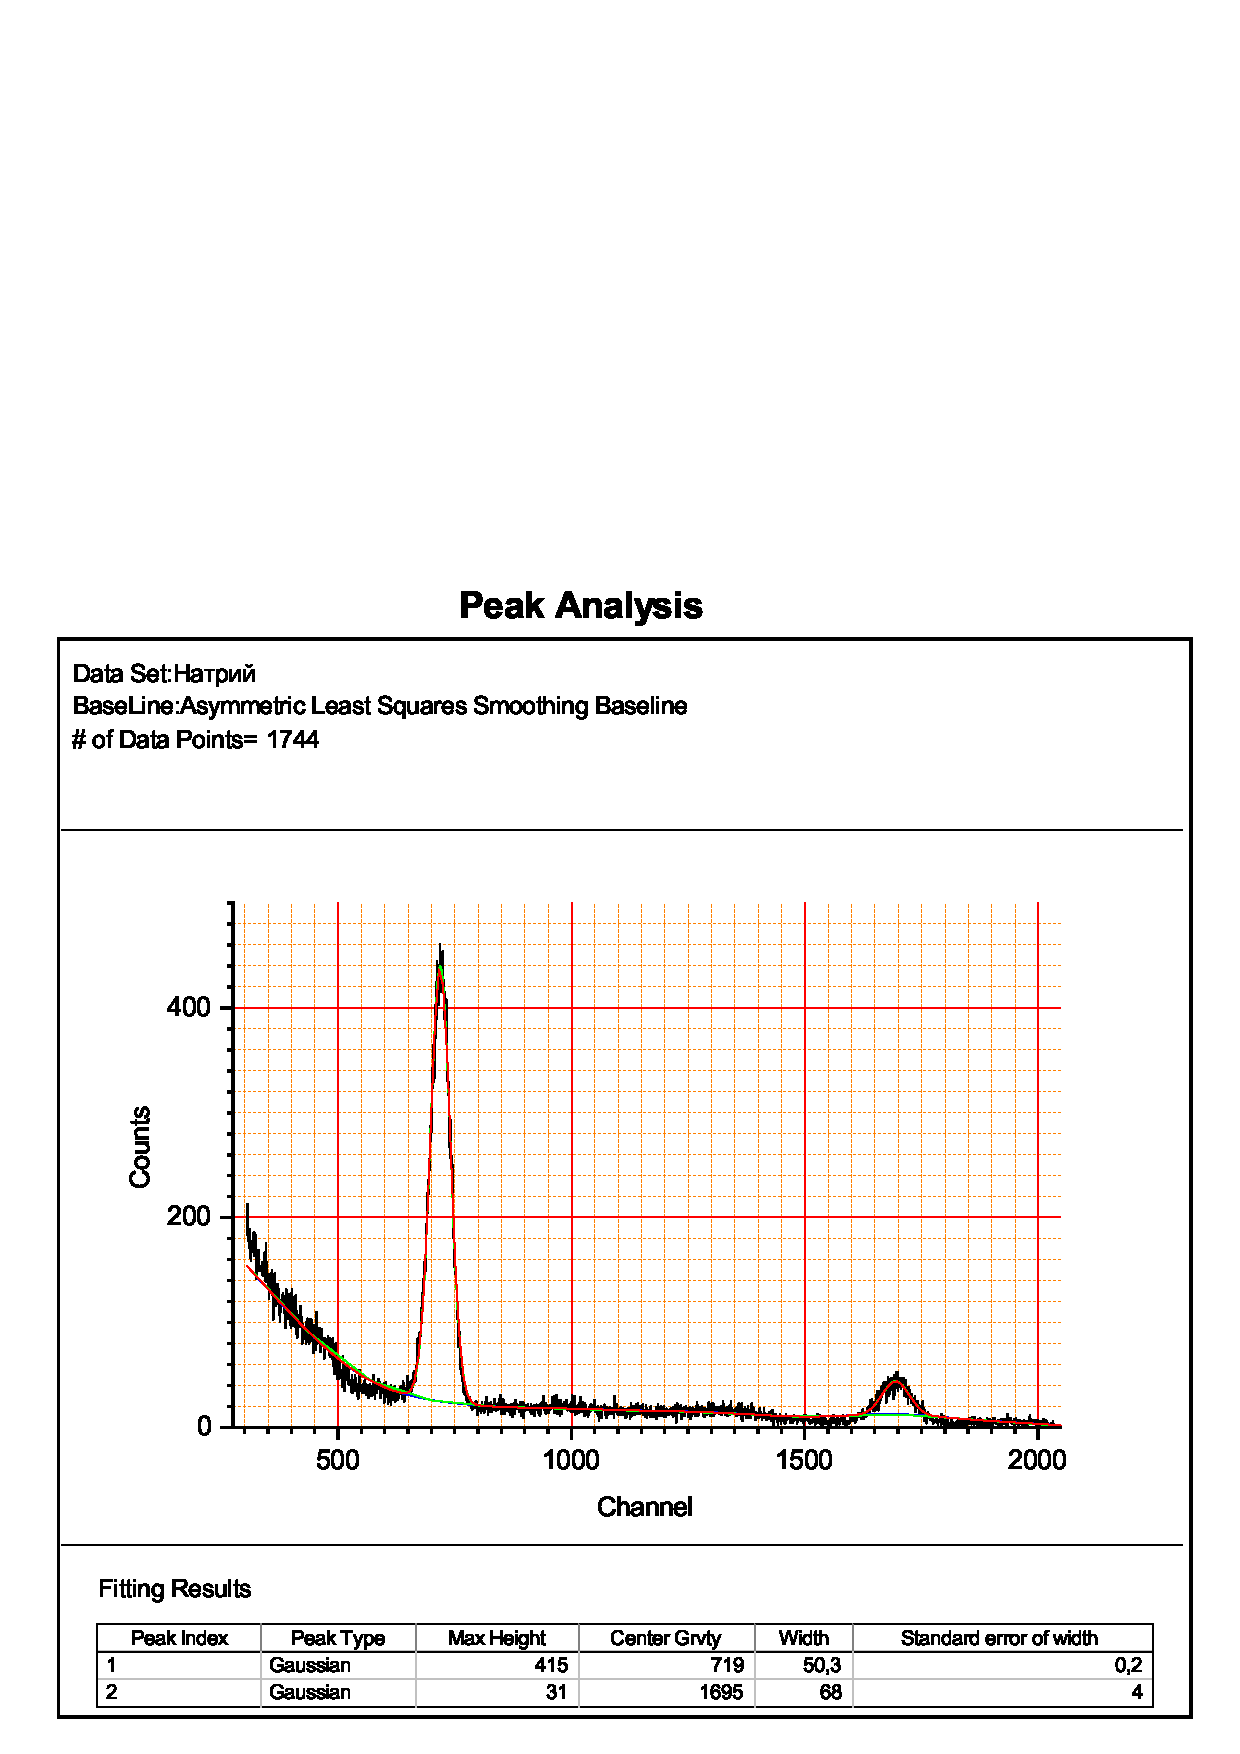
\includegraphics[width = 0.4\textwidth]{1.png}
%\end{center}
%\caption{}
%\end{wrapfigure}

%\begin{wrapfigure}{r}{0.5\textwidth}
%\begin{center}
%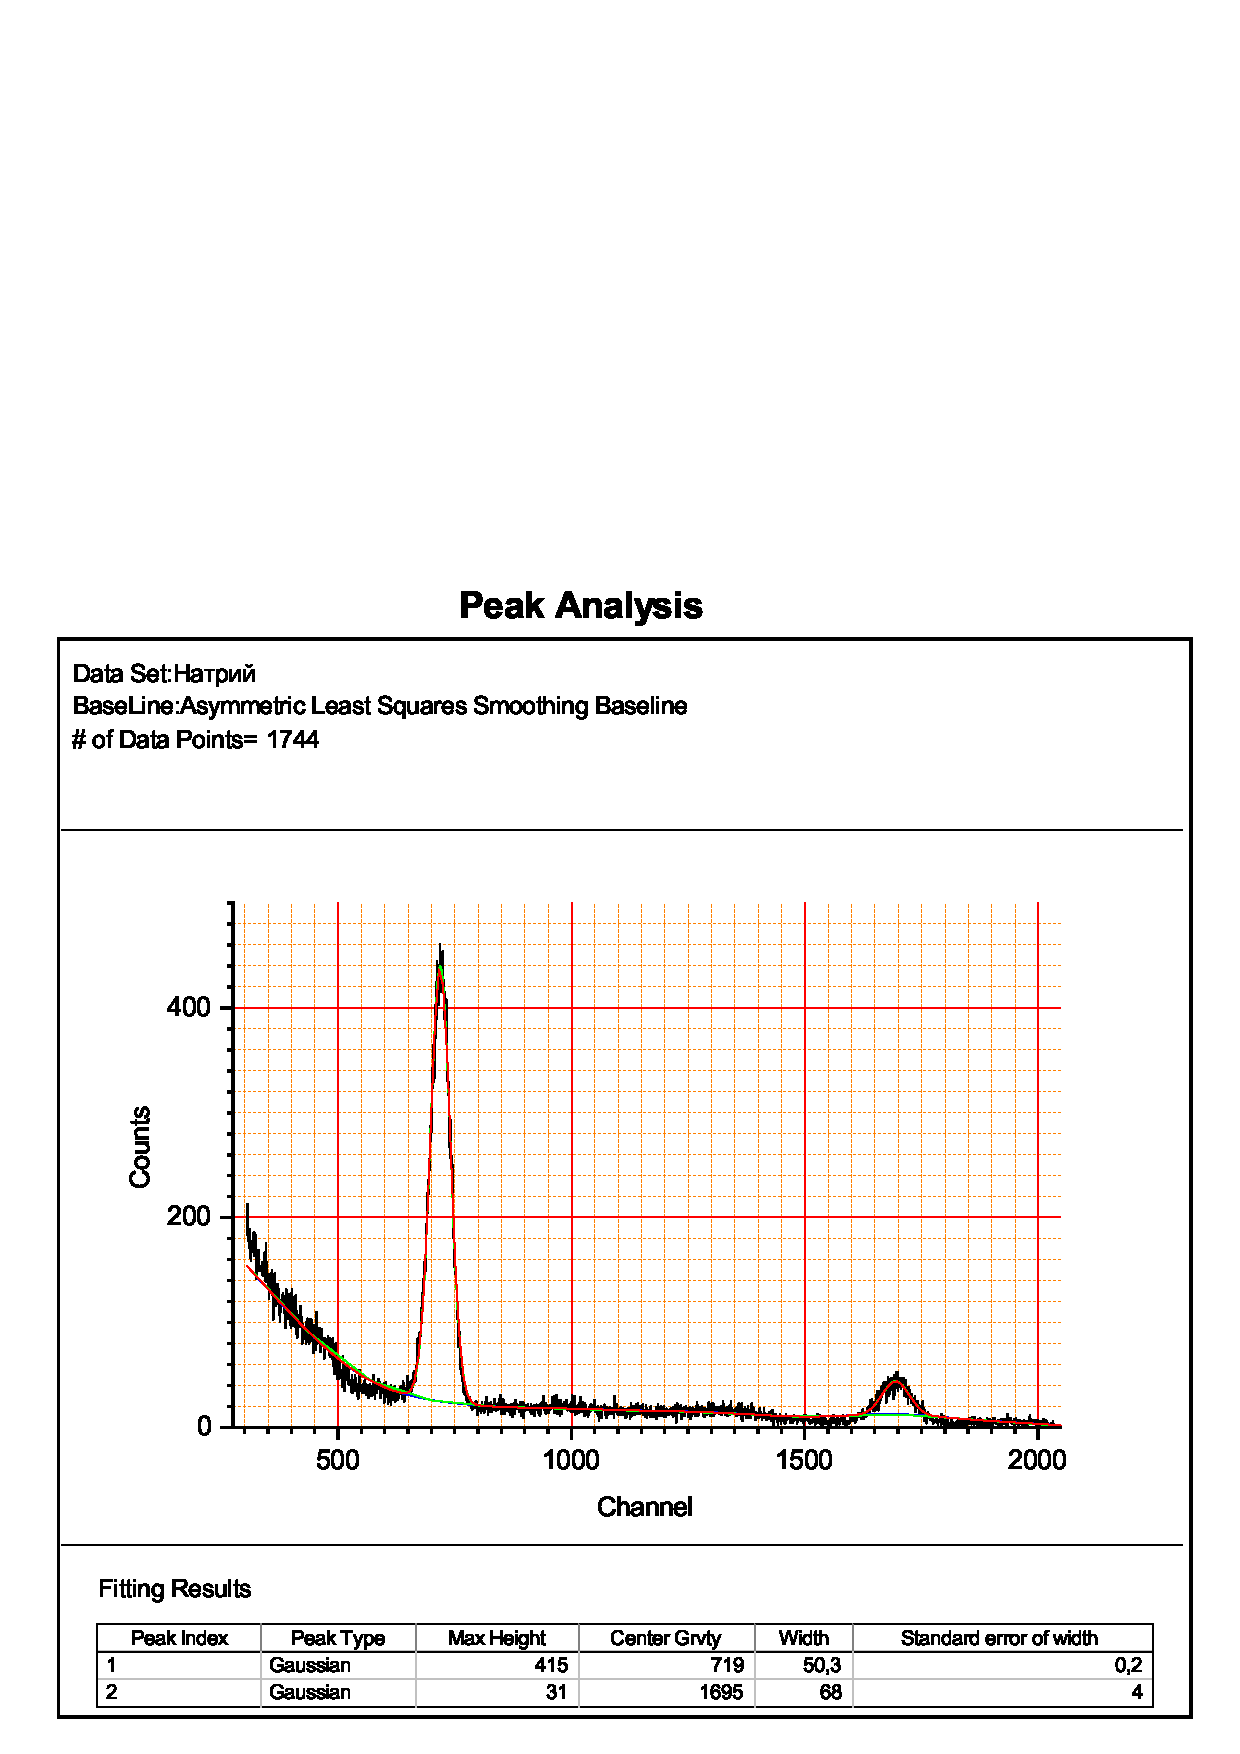
\includegraphics[width = 0.4\textwidth]{1.png}
%\end{center}
%\caption{}
%\end{wrapfigure}

\begin{document}
\maketitle
\textbf{В работе}: с помощью сцинтилляционного счётчика измеряются линейные коэффициенты ослабления потока $\gamma$-лушче в свинце, железе и алюминии; по их величине определяется энергия $\gamma$-квантов.
\section*{Теория}
Проходя через вещество, пучок $\gamma$-квантов постепенно ослабляется, ослабление происходит по экспоненциальному закону, который может быть записан в двух эквивалентных формах:
\[\begin{array}{l}
I = I_0 e^{-\mu l} ,\\
I = I_0 e^{-\mu' m_l},\\
\end{array}\]
где $I, I_0$ -- интенсивности прошедшего и падающего излучений, $l$ -- длина пути, пройденного пучком $\gamma$-лучей, $m_l$ -- масса пройденного вещества на единицу площади, $\mu$, $\mu'$ -- константы, зависящие от вещества. Ослабление потока $\gamma$-лучей возникает из-за фотоэлектрического поглощения, комптоновского рассеяния и генерации электрон-позитронных пар (при достаточных энергиях).\\
Считая, что опыт поставлен в \textit{хорошей геометрии}, то есть сквозь вещество всегда идёт узкий параллельный пучок, можно считать, что комптоновское рассеяние выводит $\gamma$-кванты из пучка и в итоге меняется количество, но не энергия $\gamma$-квантов. Это означает, что $\mu$ не зависит от $l$. Число выбывших на пути $dl$ из пучка $\gamma$-квантов
\[-dN = \mu N dl,\]
откуда
\[N = N_0 e^{\mu l},\]
или
\begin{equation}
\mu = \dfrac{1}{l} \ln \dfrac{N_0}{N}.
\end{equation}

\section*{Описание установки}
\begin{figure}[h]
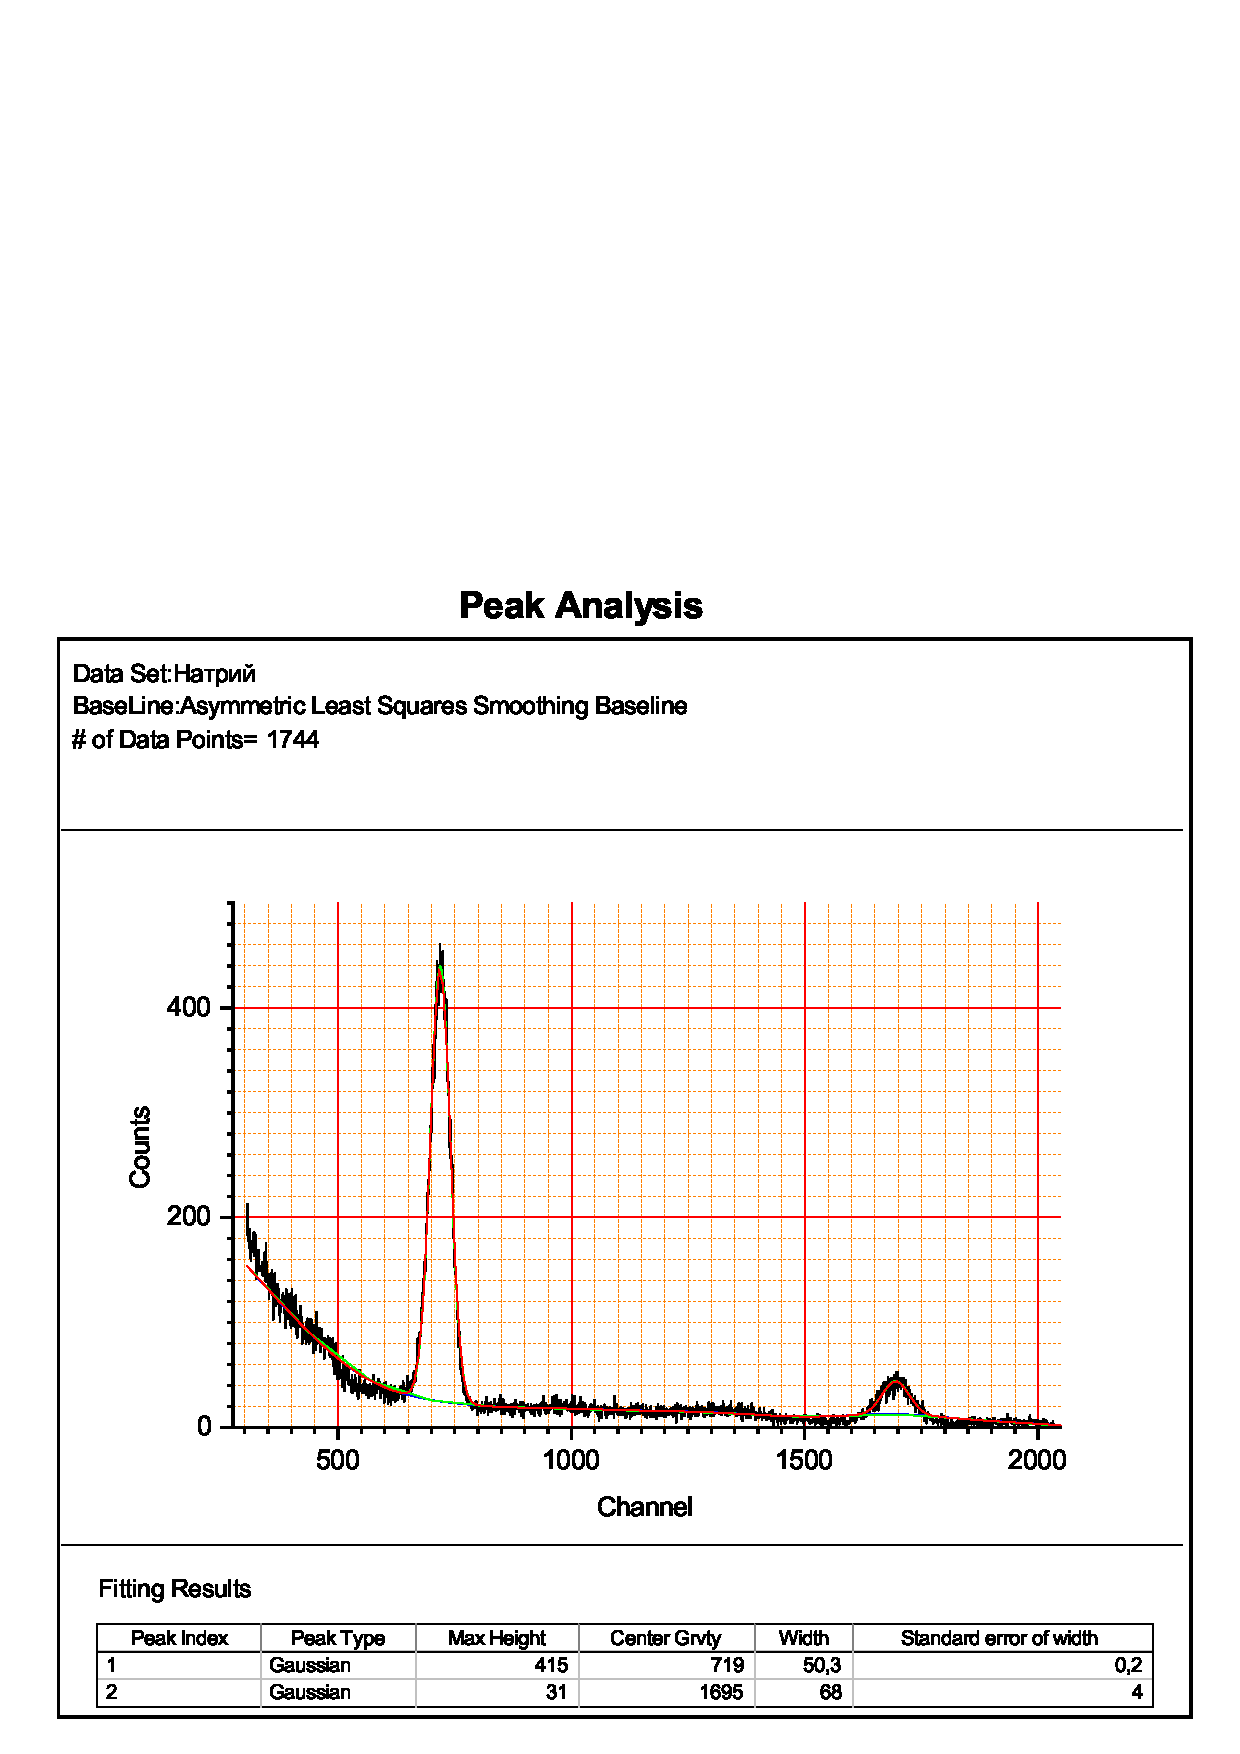
\includegraphics[scale=0.5]{1.png}
\centering
\caption{Схема установки.}
\end{figure}
На Рис. 1 изображена схема установки. Свинцовый коллиматор выделяет узкий почти параллельный пучок $\gamma$-квантов, проходящий через набор поглотителей П и регистрируемый сцинтилляционным счётчиком. Сигналы от счётчика усиливаются и регистрируются пересчётным прибором ПП. Высоковольтный выпрямитель ВВ обеспечивает питание сцинтилляционного счётчика. Чтобы уменьшить влияние плохой геометрии, счётчик расположен на большим расстоянии от источника, поглотители имеют небольшие размеры, а так же устанавливаются на расстоянии друг от друга, чтобы испытавшие комптоновское рассеяние кванты с меньшей вероятностью могли в него вернуться.
\section*{Ход работы}
Включив установку, убеждаемся в том, что она чувствует гамма-лучи: подаем на ФЭУ напряжение, указанное на установке. Измерив скорость счета при полностью открытом коллиматоре, а затем при коллиматоре, закрытом свинцовой пробкой, отметим, что скорость счета резко уменьшается (см результаты измерений), что
свидетельствует об исправности счетчика. 


Теперь исследуем поглощение $\gamma$-лучей в свинце, железе и алюминии. Для этого измеряем число частиц, попадающих в счетчик за фиксированное время, равное $t_0 = 10~\text{с}$ в отсутствие и в присутствии поглотителя. Количество поглощенных лучей измеряем для разного числа образцов -- указаны как El $\times n$, где El -- материал поглотителя, $n$ -- число поглотителей, -- а также для закрытого свинцовой пробкой коллиматора (<<Фон>>) и для коллиматора без поглотителей (<<Ничего>>). Результаты измерений представлены в Таблице 2, погрешность считаем корнем из числа частиц ($\sigma_N = \sqrt{N}$). В таблице из измерений не вычтен фон.\\
Также проведём измерения толщин поглотителей, результаты представлены в Таблице 1. Погрешность всех измерений считаем приборной $\sigma_x = 0.1~\text{см}$.
\begin{table}[h]
\begin{tabular}{|c|c|c|c|c|c|c|}
\hline
Материал & 1    & 2    & 3    & 4    & 5    & сред. \\ \hline
Pb       & 4.4  & 4.7  & 4.5  & 5.0  & 4.8  & 4.7   \\ \hline
Al       & 20.0 & 20.1 & 20.2 & 20.0 & 20.1 & 20.1  \\ \hline
Fe       & 10.1 & 10.1 & 9.8  & 10.1 & 10.1 & 10.0  \\ \hline
\end{tabular}
\centering
\caption{Измерения толщины поглотителей.}
\end{table}

\begin{table}[h!]
\begin{tabular}{|c|c|c|c|c|c|c|c|c|}
\hline
\multicolumn{2}{|c|}{}                      & 1      & 2      & 3      & 4      & 5      & 6      & сред.  \\ \hline
\multirow{2}{*}{Фон}           & $N$        & 203    & 147    & 125    & 150    & 135    & 155    & 153    \\ \cline{2-9} 
                               & $\sigma_N$ & 14     & 12     & 11     & 12     & 12     & 12     & 12     \\ \hline
\multirow{2}{*}{Ничего}        & $N$        & 234300 & 218400 & 216700 & 213700 & 212500 & 212700 & 218100 \\ \cline{2-9} 
                               & $\sigma_N$ & 500    & 500    & 500    & 500    & 500    & 500    & 500    \\ \hline
\multirow{2}{*}{Pb $\times$ 1} & $N$        & 100500 & 101800 & 103000 & 101400 & 102000 & 101300 & 101700 \\ \cline{2-9} 
                               & $\sigma_N$ & 300    & 300    & 300    & 300    & 300    & 300    & 300    \\ \hline
\multirow{2}{*}{Pb $\times$ 2} & $N$        & 48900  & 48500  & 49300  & 49000  & 48800  & 49000  & 49000  \\ \cline{2-9} 
                               & $\sigma_N$ & 200    & 200    & 200    & 200    & 200    & 200    & 200    \\ \hline
\multirow{2}{*}{Pb $\times$ 3} & $N$        & 28300  & 28400  & 28900  & 29100  & 28500  & 28900  & 28700  \\ \cline{2-9} 
                               & $\sigma_N$ & 200    & 200    & 200    & 200    & 200    & 200    & 200    \\ \hline
\multirow{2}{*}{Pb $\times$ 4} & $N$        & 15940  & 15920  & 16570  & 16380  & 16070  & 16340  & 16200  \\ \cline{2-9} 
                               & $\sigma_N$ & 130    & 130    & 130    & 130    & 130    & 130    & 130    \\ \hline
\multirow{2}{*}{Pb $\times$ 5} & $N$        & 9370   & 9210   & 9400   & 9600   & 9340   & 9400   & 9380   \\ \cline{2-9} 
                               & $\sigma_N$ & 100    & 100    & 100    & 100    & 100    & 100    & 100    \\ \hline
\multirow{2}{*}{Pb $\times$ 6} & $N$        & 5350   & 5380   & 5230   & 5460   & 5320   & 5390   & 5350   \\ \cline{2-9} 
                               & $\sigma_N$ & 70     & 70     & 70     & 70     & 70     & 70     & 70     \\ \hline
\multirow{2}{*}{Al $\times$ 1} & $N$        & 140500 & 137900 & 135900 & 134000 & 136000 & 138200 & 137100 \\ \cline{2-9} 
                               & $\sigma_N$ & 400    & 400    & 400    & 400    & 400    & 400    & 400    \\ \hline
\multirow{2}{*}{Al $\times$ 2} & $N$        & 78000  & 76600  & 77100  & 77800  & 77100  & 77600  & 77400  \\ \cline{2-9} 
                               & $\sigma_N$ & 300    & 300    & 300    & 300    & 300    & 300    & 300    \\ \hline
\multirow{2}{*}{Al $\times$ 3} & $N$        & 46700  & 47100  & 47700  & 47600  & 47800  & 47200  & 47300  \\ \cline{2-9} 
                               & $\sigma_N$ & 200    & 200    & 200    & 200    & 200    & 200    & 200    \\ \hline
\multirow{2}{*}{Al $\times$ 4} & $N$        & 29300  & 28700  & 28900  & 29500  & 29000  & 29100  & 29100  \\ \cline{2-9} 
                               & $\sigma_N$ & 200    & 200    & 200    & 200    & 200    & 200    & 200    \\ \hline
\multirow{2}{*}{Al $\times$ 5} & $N$        & 18080  & 18190  & 17910  & 18230  & 17730  & 17970  & 18020  \\ \cline{2-9} 
                               & $\sigma_N$ & 130    & 130    & 130    & 140    & 130    & 130    & 130    \\ \hline
\multirow{2}{*}{Fe $\times$ 1} & $N$        & 110900 & 109400 & 108000 & 107800 & 106400 & 105500 & 108000 \\ \cline{2-9} 
                               & $\sigma_N$ & 300    & 300    & 300    & 300    & 300    & 300    & 300    \\ \hline
\multirow{2}{*}{Fe $\times$ 2} & $N$        & 51600  & 51200  & 51400  & 51600  & 51800  & 51500  & 51500  \\ \cline{2-9} 
                               & $\sigma_N$ & 200    & 200    & 200    & 200    & 200    & 200    & 200    \\ \hline
\multirow{2}{*}{Fe $\times$ 3} & $N$        & 26300  & 26600  & 27200  & 26900  & 27200  & 29700  & 27300  \\ \cline{2-9} 
                               & $\sigma_N$ & 200    & 200    & 200    & 200    & 200    & 200    & 200    \\ \hline
\multirow{2}{*}{Fe $\times$ 4} & $N$        & 14290  & 14310  & 14380  & 14430  & 14490  & 14360  & 14380  \\ \cline{2-9} 
                               & $\sigma_N$ & 120    & 120    & 120    & 120    & 120    & 120    & 120    \\ \hline
\multirow{2}{*}{Fe $\times$ 5} & $N$        & 7700   & 7500   & 7800   & 7850   & 8150   & 7750   & 7790   \\ \cline{2-9} 
                               & $\sigma_N$ & 90     & 90     & 90     & 90     & 90     & 90     & 90     \\ \hline
\end{tabular}
\centering
\caption{Измерения числа частиц.}
\end{table}
\newpage
Построим кривые зависимости логарифма посчитанных частиц $\ln \frac{N_0}{N}$, где $N_0$ -- число частиц без поглотителей, от суммарной толщины образцов $l$. Погрешность логарифма некоторой величины $\varphi$ с погрешностью $\sigma_\varphi$ считается по формуле 
\[\sigma_{\ln \varphi} = \dfrac{\partial \ln \varphi}{\partial \varphi} \sigma_\varphi = \dfrac{\sigma_\varphi}{\varphi}.\] 
Погрешность дроби $\frac{N_0}{N}$ считаем как
\[\sigma_{\text{дробь}} = \sqrt{\dfrac{\sigma^2_{N_0}}{N^2} + \dfrac{N_0^2 \sigma_N^2}{N^4}}.\]
Графики представим на Рис. 2. Прямые имеют фиксированную точку пересечения с осями в нуле. С помощью МНК найдём коэффициент наклона прямых.\\
\begin{figure}[h]
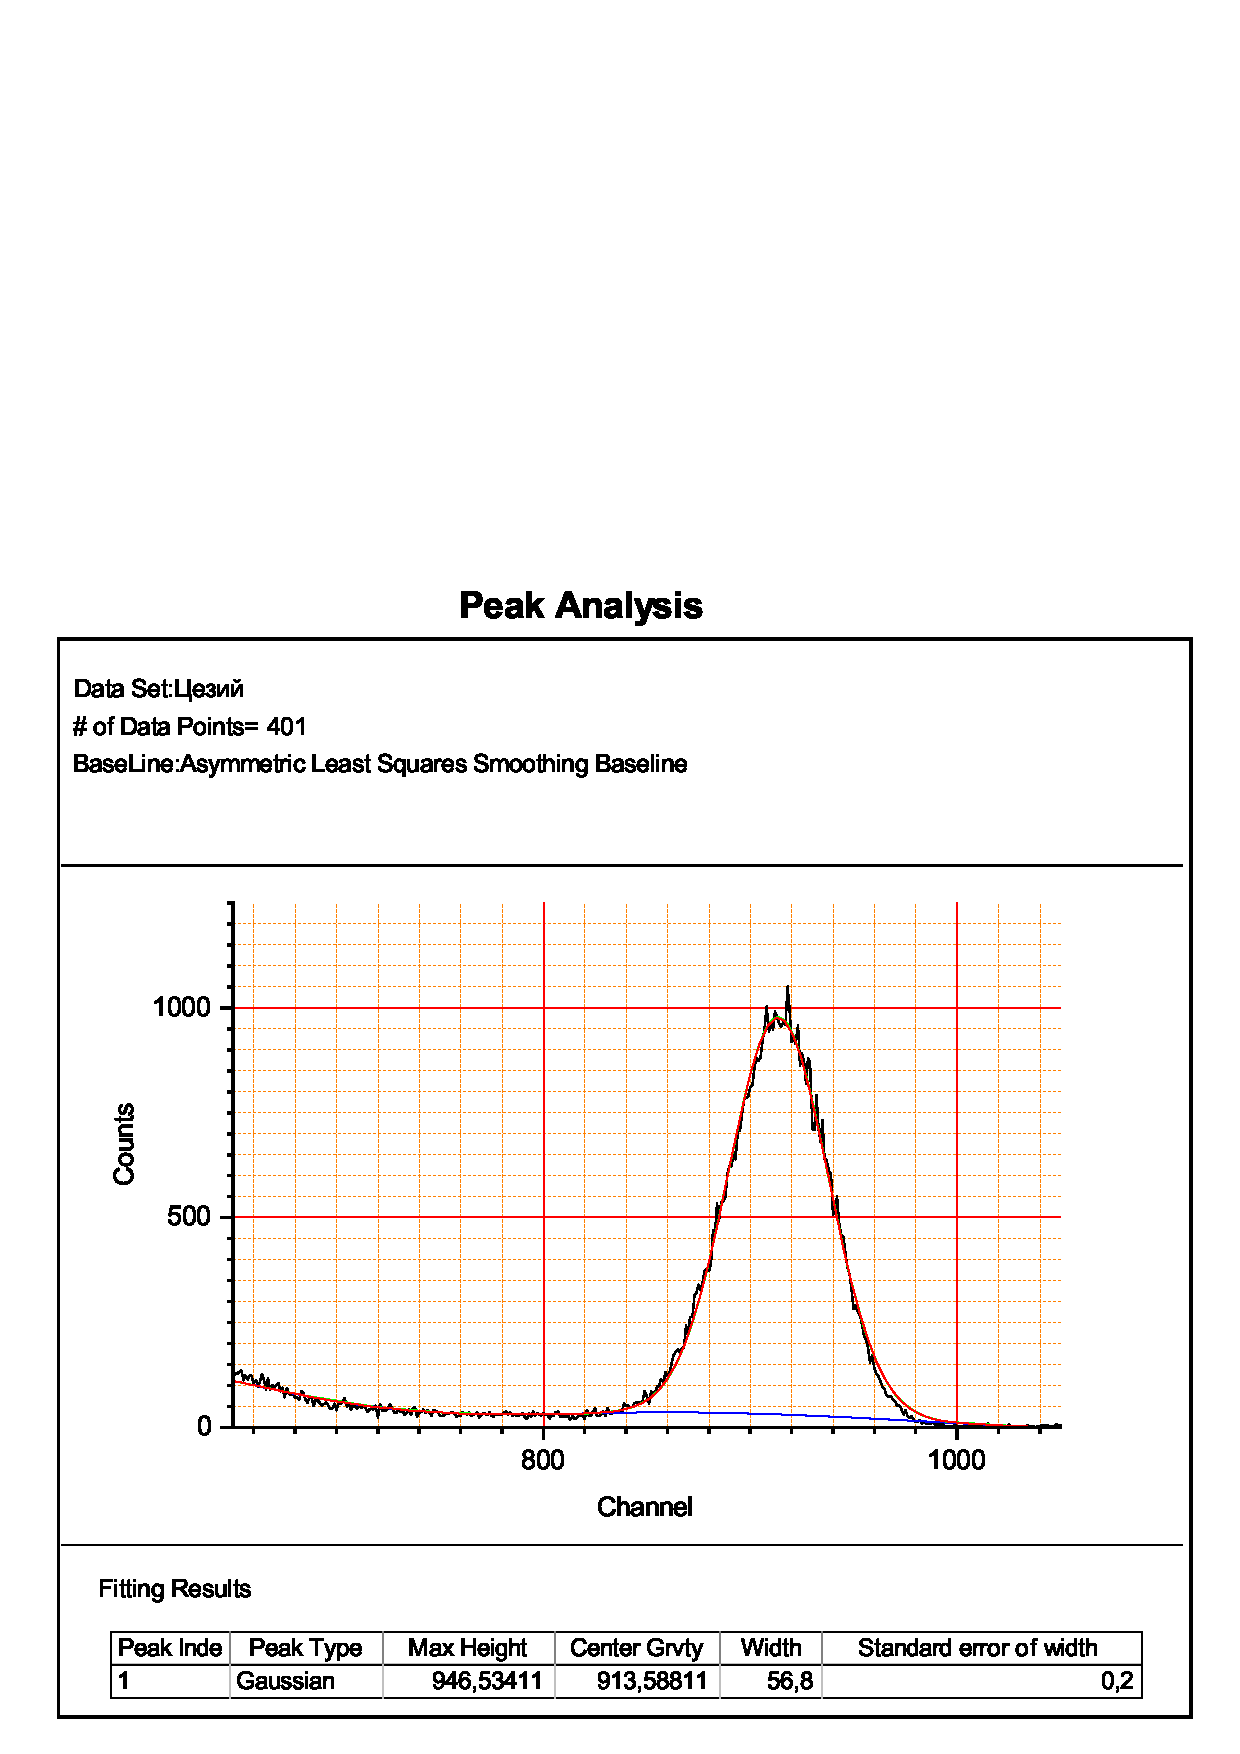
\includegraphics[scale=0.5]{3.png}
\centering
\caption{Графики $\ln \dfrac{N_0}{N} = f(l)$ для Pb (верхний-левый), Al (верхний-правый) и Fe (нижний).}
\end{figure}\\
В Таблице 3 представлены коэффициенты наклона, они же коэффициенты поглощения $\mu$, погрешность взята из МНК. По таблице в учебнике определим среднюю энергию $\gamma$-квантов в каждом опыте.
\begin{table}[h!]
\begin{tabular}{|c|c|c|c|}
\hline
   & $\mu$, $\text{см}^{-1}$ & $\sigma_\mu$, $\text{см}^{-1}$ & $E_\gamma$, МэВ \\ \hline
Pb & 1.43                    & 0.05                           & 0.60             \\ \hline
Al & 0.251                   & 0.003                          & 0.60             \\ \hline
Fe & 0.691                   & 0.009                          & 0.50             \\ \hline
\end{tabular}
\centering
\caption{Значения коэффициентов поглощения и энергия $\gamma$-квантов.}
\end{table}
\end{document}
























































